\documentclass[runningheads,envcountsame]{llncs}

\usepackage[paperwidth=15cm, paperheight=22cm, textwidth=12.2cm, textheight=19.3cm, inner=1.4cm, outer=1.4cm]{geometry}

% CODE LISTINGS
\usepackage{listings}

% GENERAL
\usepackage[T1]{fontenc}
\usepackage{array}
\newcolumntype{L}{>{$}l<{$}}
\newcolumntype{C}{>{$}c<{$}}
\newcolumntype{R}{>{$}r<{$}}
\usepackage{url}
\usepackage{amsmath}
\usepackage{amssymb}
\usepackage{stmaryrd}
\usepackage{verbatim}
\usepackage{ifthen}
\usepackage{listings}
\usepackage{graphics}

% THEOREM-LIKE ENVIRONMENTS
\spnewtheorem*{Example}{Example}{\itshape}{} 
\spnewtheorem*{Remark}{Remark}{\itshape}{} 

% FLOATS
\usepackage[font=small,labelfont=bf]{caption}
\usepackage{subfig}
\usepackage{float}
\usepackage{wrapfig}

% Mathclap macros
\def\clap#1{\hbox to 0pt{\hss#1\hss}}
\def\mathllap{\mathpalette\mathllapinternal}
\def\mathrlap{\mathpalette\mathrlapinternal}
\def\mathclap{\mathpalette\mathclapinternal}
\def\mathllapinternal#1#2{\llap{$\mathsurround=0pt#1{#2}$}}
\def\mathrlapinternal#1#2{\rlap{$\mathsurround=0pt#1{#2}$}}
\def\mathclapinternal#1#2{\clap{$\mathsurround=0pt#1{#2}$}}

% John's list
\newenvironment{johnlist}{\begin{list}{}{\itemsep=5pt \leftmargin=0pt}}{\end{list}}
\newcommand{\johnitem}[1]{\item[]\emph{#1.\ }}

% PROOFS AND INFERENCE RULES
\usepackage{mathpartir}

% FOR QUICKLY DEFINING NEW OPERATORS
\newcommand{\opbf}[1]{\mathop{\mathbf{#1}}}
\newcommand{\opsf}[1]{\mathop{\mathsf{#1}}}
\newcommand{\optt}[1]{\mathop{\mathtt{#1}}}

% SEPARATION LOGIC
\newcommand{\iterstar}[2][]{\circledast^{#1}_{#2}}
\renewcommand{\bigstar}{\circledast}
\newcommand{\magicwand}{\mathbin{{-\!\!}{*}}}
\newcommand{\septract}{\mathbin{{-\!}{\circledast}}}
\renewcommand{\star}{\mathbin{*}}
\newcommand{\Star}{\;\star\;}
\newcommand{\STAR}{\;\;\star\;\;}
\newcommand{\Pto}[1][]{\stackrel{\mbox{\scriptsize \smash{$#1$}}}\mapsto}
\newcommand{\pto}[1][]{{\Pto[#1]}}
\newcommand{\halfpto}{\pto[.5]}
\newcommand{\disjunion}{\uplus}
%\newcommand{\disjunion}{\smash{\stackrel{\smash{\raisebox{-4pt}{\smash{${\scriptsize +}$}}}}{\smash{\cup}}}}
\newcommand{\combine}{\mathop{\hspace{-1pt}\disjunion\hspace{-1pt}}}
\renewcommand{\boxed}[1]{%
  \renewcommand{\arraystretch}{0.9}%
  \mbox{\mdseries\begin{tabular}{|@{\hspace{2px}}L@{\hspace{2px}}|}\hline #1 \\ \hline \end{tabular}}%
}
\newcommand{\Boxed}[1]{%
  \renewcommand{\arraystretch}{1.0}%
  \mbox{\mdseries\begin{tabular}{|@{\hspace{2px}}L@{\hspace{2px}}|}\hline #1 \\[1.5pt] \hline \end{tabular}}%
}
\newcommand{\emp}{\mathsf{emp}}
\newcommand{\Emp}{\mathsf{Emp}}

% ARITHMETIC OPERATORS
\newcommand{\mathceil}[1]{\left\lceil#1\right\rceil}

% ASSERTIONS OPERATORS AND CONSTANTS
\newcommand{\floor}[2][R]{\left\lfloor{#2}\right\rfloor_{\hspace{-1.5pt}#1}}
\newcommand{\ceil}[2][R]{\left\lceil{#2}\right\rceil_{\hspace{-1.5pt}#1}}
\newcommand{\stab}{\mathbin{\mathsf{stab}}}
\newcommand{\entails}[1][]{\ifthenelse{\equal{#1}{}}{\models}{\models_{\mbox{\sf\scriptsize #1}}}}
\newcommand{\stronger}{\Rightarrow}
\newcommand{\STRONGER}{\;\stronger\;\;}
\newcommand{\weaker}{\Leftarrow}
\newcommand{\WEAKER}{\;\weaker\;\;}
\newcommand{\samestrength}{\Leftrightarrow}
\newcommand{\SAMESTRENGTH}{\;\samestrength\;\;}
\newcommand{\disj}{\perp}
\renewcommand{\implies}{\Longrightarrow}
\newcommand{\Implies}{\;\Longrightarrow\;}
\newcommand{\IMPLIES}{\;\;\Longrightarrow\;\;}
\newcommand{\NOTIMPLIES}{\;\;\not\Longrightarrow\;\;}
\renewcommand{\impliedby}{\Longleftarrow}
\newcommand{\Impliedby}{\;\Longleftarrow\;}
\newcommand{\IMPLIEDBY}{\;\;\Longleftarrow\;\;}
\renewcommand{\iff}{\Longleftrightarrow}
\newcommand{\Iff}{\;\Longleftrightarrow\;}
\newcommand{\IFF}{\;\;\Longleftrightarrow\;\;}
\newcommand{\eqdef}{\stackrel{\text{\tiny \rm def}}{=}}
\newcommand{\Eqdef}{\;\eqdef\;}
\newcommand{\EQDEF}{\;\;\eqdef\;\;}
\newcommand{\iffdef}{\mathop{\stackrel{\text{\tiny \rm def}}{\Leftrightarrow}}}
\newcommand{\Iffdef}{\;\mathop{\stackrel{\text{\tiny \rm def}}{\Longleftrightarrow}}\;}
\newcommand{\IFFDEF}{\;\;\mathop{\stackrel{\text{\tiny \rm def}}{\Longleftrightarrow}}\;\;}
\newcommand{\Land}{\;\wedge\;}
\newcommand{\LAND}{\;\;\wedge\;\;}
\newcommand{\Lor}{\;\vee\;}
\newcommand{\LOR}{\;\;\vee\;\;}
\newcommand{\union}{\cup}
\newcommand{\intersect}{\cap}
\newcommand{\strachey}[1]{\llbracket #1 \rrbracket}
\newcommand{\id}{\mathsf{id}}
\newcommand{\Id}{\mathsf{Id}}
\newcommand{\true}{\mathsf{true}}
\newcommand{\false}{\mathsf{false}}
\newcommand{\True}{\mathsf{True}}
\newcommand{\False}{\mathsf{False}}
\newcommand{\parallelfunc}[2]{\mathbin{{_{#1}}\hspace{-1.5pt}\parallel\hspace{-1.2pt}{_{#2}}}}

% PROGRAMMING LANGUAGE
\newcommand{\ang}[1]{\langle #1 \rangle}
\newcommand{\prov}[1][]{\ifthenelse{\equal{#1}{}}{\vdash}{\vdash_{\mbox{\sf\scriptsize #1}}}}
\newcommand{\hook}[1]{\smash{\stackrel{\makebox[0pt][c]{\raisebox{2pt}{$\leftharpoonup$}}}{\smash{#1}}}}
\newcommand{\mathbi}[1]{\mbox{\bfseries \itshape #1}}
\newcommand{\pow}{\mathcal{P}}
\newcommand{\fv}{\mathop{\mathrm{fv}}}
\newcommand{\dom}{\mathop{\mathrm{dom}}}
\newcommand{\mods}{\mathop{\mathrm{mods}}}

% PROGRAMMING LANGUAGE
\renewcommand{\colon}{\opbf{:}}
\renewcommand{\parallel}{\opsf{ll}}
\newcommand{\semicolon}{\opbf{;}}
\newcommand{\Skip}{\mathop{\mathtt{skip}}}
\newcommand{\assign}[2]{\ensuremath{#1}\mathop{\texttt{:=}}\ensuremath{#2}}
\newcommand{\assert}{\optt{assert}}
\newcommand{\assume}{\optt{assume}}

% SPECIFICATIONS
\newcommand{\ass}[1]{{%
%\color{blue}%
\left\{\mbox{\mdseries\begin{tabular}{@{}L@{}}#1\end{tabular}}\right\}}}
\newcommand{\pspec}[6][]{#4,#5\prov[#1]\{#3\}\,#2\,\{#6\}}
\newcommand{\Pspec}[6][]{#4,#5\prov[#1]\ass{#3}\,#2\,\ass{#6}}
\newcommand{\modspec}[5][]{#4\prov[#1]\ass{#3}\,#2\,\ass{#5}}
\newcommand{\sspec}[6][]{#4,#5\entails[#1]\{#3\}\,#2\,\{#6\}}
\newcommand{\seqspec}[3]{\{#1\}\,#2\,\{#3\}}
\newcommand{\pp}{\mathbi{p}}
\newcommand{\qq}{\mathbi{q}}
\renewcommand{\r}{\mathbi{r}}
\newcommand{\R}{\mathbb{R}}
\newcommand{\univ}{\mathbb{U}}
\newcommand{\x}{{\tt x}}
\newcommand{\y}{{\tt y}}
\newcommand{\Rinc}[1]{R_{#1{\texttt{+}}}}
\newcommand{\Ginc}[1]{G_{#1{\texttt{+}}}}

% MALLOC PROOF
\newcommand{\malloc}{{\tt malloc}}
\newcommand{\sbrk}{{\tt sbrk}}
\newcommand{\free}{{\tt free}}
\newcommand{\ls}[2][]{#1 {\twoheadrightarrow} #2}
\newcommand{\block}[2]{\mathop{\mathit{block}}(#1,#2)}
\newcommand{\arena}{\mathop{\mathit{arena}}}
\newcommand{\token}{\mathop{\mathit{token}}}
\newcommand{\arenatoken}{\mathop{\mathit{arenatoken}}}
\newcommand{\A}[2][]{#1 {\smash{\underset{\raisebox{3.5pt}{\smash{\sf\scriptsize a}}}{\rightarrow}}} #2}
\newcommand{\U}[2][]{#1 {\smash{\underset{\raisebox{3.5pt}{\smash{\sf\scriptsize u}}}{\rightarrow}}} #2}
\newcommand{\B}[2][]{#1 {\rightarrow} #2}
\newcommand{\E}[2]{#2 {\raisebox{2pt}{$\curvearrowleft$}} #1}
\newcommand{\s}{{\tt s}}
\renewcommand{\t}{{\tt t}}
\newcommand{\temp}{{\tt temp}}
\newcommand{\p}{{\tt p}}
\newcommand{\q}{{\tt q}}
\newcommand{\brk}{\mathop{\mathit{brk}}}
\newcommand{\ret}{{\tt ret}}
\newcommand{\n}{{}\\{} \hfill }
\newcommand{\nw}{{\tt nw}}
\newcommand{\ap}{{\tt ap}}
\newcommand{\nbytes}{{\tt nbytes}}
\newcommand{\WORD}{{\tt WORD}}
\newcommand{\amp}{\mbox{\tt\&}}
\newcommand{\busy}[1]{\ensuremath{#1_{\mathrm{busy}}}}

\title{Explicit Stabilisation \\ for Modular Rely-Guarantee Reasoning}
\author{John Wickerson, Mike Dodds and Matthew Parkinson}
\institute{University of Cambridge Computer Laboratory}

\begin{document}

%\pagestyle{plain}

\maketitle

\begin{abstract}
We propose a new formalisation of stability for Rely-Guaran\-tee, in which an assertion's stability is encoded into its syntactic form. This allows two advances in modular reasoning. Firstly, it enables Rely-Guarantee, for the first time, to verify concurrent libraries independently of their clients' environments. Secondly, in a sequential setting, it allows a module's internal interference to be hidden while verifying its clients. We demonstrate our approach by verifying, using RGSep, the Version~7 Unix memory manager, uncovering a twenty-year-old bug in the process.
\end{abstract}

\section{Introduction}

Reasoning about concurrent programs is hard because commands from different threads are interleaved non-deterministically. With many threads and many commands per thread, na�ve reasoning soon succumbs to a combinatorial explosion. The Rely-Guarantee (RG) method \cite{cliff_thesis} restores tractability through abstraction. In addition to the pre and postconditions inherited from Hoare logic \cite{hoarelogic}, a command is specified by two relations between states: a \emph{rely} $R$ that specifies all the state transitions (or `actions') the environment can cause, and a \emph{guarantee} $G$ that specifies all the actions of the command itself. (The environment is the set of concurrently-running threads.) The method conservatively assumes that between consecutive commands in a thread, any number of actions in $R$ may occur. The truth of an assertion that holds after one command must be preserved by this `interference', so that it may be safely assumed by the next command. Such an assertion is deemed \emph{stable under} $R$.

Stability is traditionally enforced through side-conditions on proof rules. We propose (Sect.~\ref{sect:expstab}) a new formalisation in which stability is recorded within the syntactic form of the assertion itself. Just as `explicit substitution' \cite{explicit_substitutions} added substitution to the syntax of $\lambda$-calculus terms, our work adds stabilisation to the syntax of RG assertions. We propose two new constructs: $\floor{p}$ to denote the weakest assertion that is both stronger than $p$ and stable under $R$, and dually, $\ceil{p}$ to denote the strongest stable assertion that is weaker than $p$.

The main benefit is in modularity, two forms of which we tease apart and tackle separately: verifying concurrent libraries independently of clients, and verifying clients of a (sequential) module independently of its implementation.
\begin{johnlist}
\johnitem{\hspace{-1.5pt}Verifying libraries independently of clients} RG is a compositional meth\-od: an entire program's proof depends only upon the proofs of its constituent commands. Yet it is not modular: a command's proof cannot necessarily be re-used when the command features in a different program, because proofs are environment-specific. Thus, RG cannot verify libraries that are invoked in several different environments. Our solution (Sect.~\ref{sect:modularity_solution}) has the library record stability requirements using $\floor{\ }$ and $\ceil{\ }$, but leave the specification parametric in $R$. Each client then instantiates $R$ appropriately and performs the stabilisation.
\johnitem{\hspace{-1.5pt}Verifying clients independently of module implementations} In Sect.~\ref{sect:rgsep}, we bring explicit stabilisation to an RG-style logic that reasons about heap-manipulating programs: RGSep \cite{rgsep}. Because it divides the heap into both thread-local and shared regions, RGSep's notion of stability is more complex than that of ordinary RG; in particular, while only the shared heap is susceptible to interference, we shall see that the local heap can still affect stability arguments. Originally conceived for concurrency, RGSep is apt for verifying sequential modules too. Such a verification must consider every action by which a client can mutate the module's part of the heap. Our extension of explicit stabilisation to RGSep permits an {\sc InfoHiding} rule that allows this so-called `internal interference' to be hidden while verifying clients. We demonstrate (Sect.~\ref{sect:malloc}) this approach by verifying -- for the first time -- the Version~7 Unix memory manager. In doing so, we uncover a bug that has lain dormant since 1979.
\end{johnlist}
We begin with a short introduction to the RG proof system, followed by a brief account of the failure of traditional RG to provide a modular specification for even one of the most trivial library functions: increment.


\section{Background: Rely-Guarantee reasoning}\label{sect:rgbackground}

RG specifications are of the form $\pspec CpRGq$, where $R$ and $G$ are relations between states. Following \cite{rg:nieto}, $G$ shall be reflexive. This specification expresses that when $C$ begins execution in a state satisfying the precondition $p$, in an environment whose interference is limited to the actions in the rely $R$, then any state transitions performed by $C$ are within its guarantee $G$, and moreover, if the execution terminates, the final state satisfies the postcondition $q$.

\begin{figure}[tb]
\vspace{-6pt}
  \begin{mathpar}
    \inferrule[Weaken]{\pspec C{p'}{R'}{G'}{q'} \\\\ p\stronger p' \\ q'\stronger q \\\\ R\subseteq R' \\ G'\subseteq G }
    {\pspec CpRGq}
    \and
    \inferrule[Par]{\pspec{C_1}{p_1}{R \union G_2}{G_1}{q_1} \\ \pspec{C_2}{p_2}{R \union G_1}{G_2}{q_2}}
    {\pspec{C_1 \parallel C_2}{p_1\land p_2}{R}{G_1\union G_2}{q_1\land q_2}}
    \and
    \inferrule[Basic]{ \prov \seqspec pcq \\ \hook p \intersect c \subseteq G \\\\ p \stab R \\ q \stab R }
    {\pspec cpRGq}
    \and
    \inferrule[Skip]{p \stab R} {\pspec {\Skip}pRGp}
    \and
    \inferrule[Loop]{\pspec CpRGp }
    {\pspec{C^+}pRGp}
  \end{mathpar}
\vspace{-12pt}
  \caption{Selected RG proof rules (with stability checks)}
  \label{fig:rgrules_before}
\end{figure}

Figure~\ref{fig:rgrules_before} presents a selection of the RG proof rules, which concern commands of the following simple parallel language:
\[C ::= \Skip \mid C\semicolon C \mid C \parallel C \mid C+C \mid C^+ \mid c\]
The + operator chooses one of its operands to execute, while $C^+$ executes $C$ at least once.\footnote{Interestingly, a variant of the {\sc Loop} rule for reasoning about $C^*$ commands would require a stability check on $p$, in case $C^*$ should behave like $\Skip$. Our language uses $C^+$ so as to sidestep this check.} We consider only partial correctness, so these non-deterministic constructs for choice and looping suffice for encoding {\tt if} and {\tt while} commands. The language is parameterised on the set of basic commands $c$, which are relations that model atomic state transformations. We shall assume $c$ includes {\tt assert} and {\tt assume} commands and variable assignment. See \cite{tr} for the complete set of proof rules and the formal semantics of our language.

The {\sc Basic} rule requires that $c$ meets the sequential specification $\seqspec pcq$, and that any action it performs is within its guarantee. It uses the notation $\hook p \eqdef \{(\sigma,\sigma')\mid \sigma\entails p\}$. The pre and postconditions of the two `ground' commands, $c$ and $\Skip$, are required to be stable. Since the other commands are built inductively from these, their rules can assume any inherited assertions to be stable (or else derived from stable assertions by the {\sc Weaken} rule). Stability checks are notated as follows:

\begin{definition}[Stability]\label{defn:stability}
  $p\stab R \Eqdef \forall\sigma,\sigma'\ldotp \sigma\entails p \Land R(\sigma, \sigma') \Implies \sigma'\entails p$.
\end{definition}

The {\sc Par} rule marks the epitome of RG reasoning. When reasoning about commands composed in parallel, the rely of each command is extended to include the guarantee of the other. The composed command $C_1\parallel C_2$ guarantees actions in either of its components' guarantees, and establishes both components' postconditions upon completion.

\subsection{The problem with verifying libraries}\label{sect:modularity_problem}

Consider a library function {\tt f()} that atomically increments a shared variable \x. Its two clients, {\tt g()} and {\tt h()}, invoke {\tt f()} in an empty environment and an environment that may increase \x, respectively. Call this latter environment $\Rinc{\x}$. The guarantee $\Ginc{\x}$ additionally dictates that no variable other than \x\ changes.
\begin{definition}\label{defn:fgh}
\emph{$\begin{array}[t]{rcl}
\texttt{f()} &\EQDEF& \texttt{x++} \\
\texttt{g()} &\EQDEF& \assume(\x{=}3)\semicolon\ \texttt{f()}\semicolon\ \assert(\x{=}4) \\
\texttt{h()} &\EQDEF& \assume(\x{=}5)\semicolon\ (\texttt{f()} \parallel \texttt{f()})\semicolon\ \assert(\x{\ge}6) \\
\Rinc{\x} &\EQDEF& \{(\sigma,\sigma')\mid \sigma(\x)\le\sigma'(\x)\} \\
\Ginc{\x} &\EQDEF& \{(\sigma,\sigma')\mid \sigma(\x)\le\sigma'(\x) \Land \forall v\neq\x\ldotp \sigma(v)=\sigma'(v)\}
\end{array}$}
\end{definition}
Now, the proofs of {\tt g()} and {\tt h()} hinge, respectively, upon deriving the following two specifications for {\tt f()}:
\[
\pspec{\texttt{f()}}{\x{=}X}{\emptyset}{\Ginc{\x}}{\x{=}X{+}1} \qquad\qquad
\pspec{\texttt{f()}}{\x{\ge}X}{\Rinc{\x}}{\Ginc{\x}}{\x{\ge}X{+}1}
\]
Both hold, yet no single `most general' specification can derive them both. The first has the stronger postcondition but the smaller rely; the second is vice versa. This troublesome tradeoff can be blamed on stability: the larger the rely, the tougher the stability requirement, and thus, the weaker the postcondition.

In Sect.~\ref{sect:modularity_solution}, we shall present a single specification for {\tt f()} from which both of the above can be derived. Parameterised on an arbitrary rely $R$, it simply states that the postcondition needs weakening from $\x{=}X{+}1$ just enough to become stable under $R$. Upon instantiating $R$ to $\Rinc{\x}$, to verify {\tt h()}, the postcondition becomes $\x{\ge}X{+}1$. And when $R$ is $\emptyset$, for {\tt g()}'s proof, no weakening is required.

\section{Explicit Stabilisation}\label{sect:expstab}

This section describes our formalisation of stability and applies it to the RG proof rules. The remaining sections develop two alternate proof systems: one (Sect.~\ref{sect:modularity_solution}) that can specify libraries independently of clients, and another (Sects.~\ref{sect:rgsep} and~\ref{sect:malloc}) that lets a module hide from clients its internal interference.

We propose two new syntactic constructs: $\floor{p}$ for the weakest assertion that is stronger than $p$ and stable under $R$, and $\ceil{p}$ for the strongest assertion that is weaker than $p$ and stable under $R$. That is, $\floor{p} = \bigvee\{q\mid q\stronger p \land q\stab R\}$ and $\ceil{p} = \bigwedge\{q\mid q\weaker p \land q\stab R\}$.
\begin{definition}[Semantics of $\floor{p}$ and $\ceil{p}$]\label{defn:floorceil} The required properties are realised uniquely by the following constructions:\vspace{-3pt} 
\[\begin{array}{rcl}
\sigma\entails \floor{p} &\IFFDEF& \ \forall \sigma'\ldotp (\sigma,\sigma')\in R^* \implies \sigma'\entails p \\[3pt]
\sigma\entails \ceil{p} &\IFFDEF& \ \exists \sigma'\ldotp (\sigma',\sigma)\in R^* \land \sigma'\entails p.
\end{array}\]
\end{definition}

\begin{wrapfigure}{R}{43mm}
\vspace{-33pt}
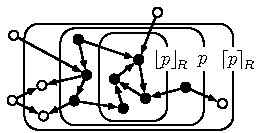
\includegraphics{arrowdiagram.pdf}
\vspace{-20pt}
\caption{}
\label{fig:arrowdiagram}
\vspace{-15pt}
\end{wrapfigure}

Figure~\ref{fig:arrowdiagram} presents the intuition behind our new
operators. The nodes represent states; those that are filled satisfy
some assertion $p$. The edges depict transitions of an arbitrary rely $R$. The states in $\floor{p}$ are those from which any reachable state satisfies $p$. The states in $\ceil{p}$ are those reachable from a state in $p$.

Our operators can also be defined using Dijkstra's predicate
transformer semantics \cite{dijkstrabook}: $\floor{p}$ is the weakest
precondition of $R^*$ given postcondition $p$, while $\ceil{p}$ is the strongest postcondition of $R^*$ given precondition $p$.

\begin{Example} We stabilise $\x{=}0$ and $\x{\ne}0$ under $\Rinc{\x}$ (see Definition~\ref{defn:fgh}) like so:\vspace{-3pt}
\[
\floor[\Rinc{\x}]{\x{=}0} \!\samestrength\, \false \hspace{13pt} 
\ceil[\Rinc{\x}]{\x{=}0} \!\samestrength\, \x{\ge}0 \hspace{13pt} 
\floor[\Rinc{\x}]{\x{\ne}0} \!\samestrength\, \x{>}0 \hspace{13pt} 
\ceil[\Rinc{\x}]{\x{\ne}0} \!\samestrength\, \true
\]
\end{Example}

\subsection{Properties of explicit stabilisation}\label{sect:stabprops} Both $\floor[]{\ }$ and $\ceil[]{\ }$ are monotonic with respect to $\stronger$. They are related via the equivalence $\floor[R]{\neg p} \samestrength \neg \ceil[R^{-1}]{p}$. Each has no effect on an already-stable operand, or when $R$ is empty. Both $\true$ and $\false$ are stable, and conjunction and disjunction both preserve stability. The distributivity properties of $\floor[]{\ }$ and $\ceil[]{\ }$ over $\land$ and $\lor$ are analogous to those of $\forall$ and $\exists$ respectively:
\[
\begin{array}{rclrcl}
\floor{p \land q} &\SAMESTRENGTH& \floor{p} \land \floor{q} & \hspace{40pt} \floor{p \lor q} &\WEAKER& \floor{p} \lor \floor{q} \\[3pt]
\ceil{p \land q} &\STRONGER& \ceil{p} \land \ceil{q} & \hspace{40pt}
\ceil{p \lor q} &\SAMESTRENGTH& \ceil{p} \lor \ceil{q}
\end{array}
\]
Several properties mirror those of the floor and ceiling functions in arithmetic, from which our syntax is borrowed. If $R\subseteq R'$, we have:
\[
\begin{array}{l} \floor[R']{\floor[R]{p}} \SAMESTRENGTH\! \floor[R]{\floor[R']{p}} \SAMESTRENGTH\! \ceil[R]{\floor[R']{p}} \SAMESTRENGTH\! \floor[R']{p} \\[3pt]
\ceil[R']{\ceil[R]{p}} \SAMESTRENGTH\! \ceil[R]{\ceil[R']{p}} \SAMESTRENGTH\! \floor[R]{\ceil[R']{p}} \SAMESTRENGTH\! \ceil[R']{p}
\end{array}
\]
Finally, the following property reminds us of the trade-off mentioned in Sect.~\ref{sect:modularity_problem}: that as the rely becomes more permissive, stability becomes harder to show:
\[
R \subseteq R' \text{ implies } \floor[R]{p} \weaker \floor[R']{p} \text{ and } \ceil[R]{p} \stronger \ceil[R']{p}
\]

\subsection{Application to RG proof rules}\label{sect:stab_rg}

\begin{wrapfigure}{R}{43mm}
\small
\vspace{-34pt}
\begin{mathpar}
    \inferrule[Basic-S]{\prov \seqspec pcq \\ \hook p \intersect c \subseteq G }
    {\pspec{c}{\floor{p}}{R}{G}{\ceil{q}}}
    \and
    \inferrule[Skip-S]{ }{\pspec{\Skip}pRG{\ceil{p}}}
  \end{mathpar}
\vspace{-10pt}
\caption{ New RG proof rules (with stabilised assertions)}
\label{fig:rgrules_after}
\vspace{-10pt}
\end{wrapfigure} 

We now describe how the RG proof rules (Fig.~\ref{fig:rgrules_before}) can be adapted to use explicit stabilisation rather than side-conditions.

Figure \ref{fig:rgrules_after} displays the replacements for the {\sc Basic} and {\sc Skip} rules; the others remain unchanged. The {\sc Basic-S} rule first derives $p$ and $q$ by considering $c$ sequentially; that is, without concern for stability. A concurrent specification is obtained by strengthening $p$ and weakening $q$ until they are both stable. The {\sc Skip-S} axiom is justified by considering the execution of $\Skip$ from an initial state satisfying $p$. This state also satisfies $\ceil{p}$, and the final state must too, since $\Skip$ does nothing. The following backward-reasoning alternative is interderivable: $\pspec{\Skip}{\floor{p}}RGp$.

The new rules are at least as powerful as the originals, which can be obtained by restoring the stability checks and then removing the redundant stabilisations.

\subsection{Aside: Simplification of complex RG proof rules}\label{sect:exp_decomp}

We now highlight the elegance of explicit stabilisation by showing how it can simplify and generalise complex RG proof rules that rely subtly upon stability. 

Coleman \cite{exp_decomp} proposes the following rule for reasoning about one-armed conditional statements whose test conditions are evaluated non-atomic\-ally in the presence of interference.
\[
\inferrule{\opsf{StableExpr}(e_s, R) \\ \pspec C{p\land e_s}RGq \\ \opsf{SingleUnstableVar}(e_u, R) \\ \forall \sigma,\sigma'\ldotp \sigma\entails p \land (\sigma,\sigma')\in R^* \land \sigma'\entails\neg(e_s\land e_u) \implies \sigma'\entails q \\ \{\neg e_u, p, q\} \stab R}{ \pspec{\texttt{if } e_u \land e_s \texttt{ then } C}pRGq }
\]
Tests are pure, and comprise an unstable conjunct $e_u$ and a `stable' conjunct $e_s$ that contains no variables that $R$ can change (first premise). Crucially, only $e_s$ can be assumed still to hold by $C$ (second premise). By requiring $e_u$ to involve only a single read of an unstable variable (third premise), we can treat it as a predicate of a single state -- the state in which the read occurs -- despite not knowing which state that is. Should the test fail, the postcondition must be met without evaluating $C$ (fourth premise). That premise requires $R$ to preserve the falsity of $e_u$ (fifth premise) so as to ensure that the obligation to fulfil $q$ cannot be bypassed by having the test evaluate to {\tt false} but later become logically $\true$.

Now consider the following alternative rule, which uses explicit stabilisation.
\[
\inferrule{\mbox{$\begin{array}{l} \  \\ \opsf{SingleUnstableVar}(e, R) \qquad \{p, q\} \stab R \end{array}$} \\ \mbox{$\begin{array}{l} \pspec{C_1}{p\land \ceil{e}}RGq \\ \pspec{C_2}{p\land \ceil{\neg e}}RGq \end{array}$} }{ \pspec{\texttt{if } e \texttt{ then } C_1 \texttt{ else } C_2}pRGq }
\]
Essentially, the execution of $C_1$ begins in a state that is reachable (by a sequence of environment actions) from one in which $e$ evaluated to {\tt true}. Similarly, $\ceil{\neg e}$ describes a state reached from one where $e$ did not hold. Stability checks on $p$ and $q$ remain only for compatibility with the rest of Coleman's system.

Thanks to explicit stabilisation, the new rule has fewer and simpler premises, plus it extends naturally to two-armed conditionals. Moreover, $e$ need not be split into stable and unstable conjuncts, for our rule handles arbitrary test conditions.


\section{Verifying concurrent library code}\label{sect:modularity_solution}

\newcommand{\lm}{\mathop{\mathit{lm}}}

Equipped with a notation for stabilising assertions, we revisit the challenge we set in Sect.~\ref{sect:modularity_problem}: to verify concurrent library code using RG reasoning.

Recall our library function {\tt f()} and its clients {\tt g()} and {\tt h()} from Definition~\ref{defn:fgh}. Using explicit stabilisation, we can derive the following specification, which is parametric in $R$ (although its instantiation will be restricted, as described shortly).
\[
\pspec{\texttt{f()}}{\ceil{\x{=}X}}{R}{\Ginc{\x}}{\ceil{\x{=}X{+}1}}
\]
Observe that instantiating $R$ to $\emptyset$ yields a specification suitable for proving {\tt g()}, while {\tt h()} can be proved having set $R$ to $\Rinc{\x}$. We now present a proof system for such `parametric specifications' and formally derive the above one for {\tt f()}.

In a parametric specification, the rely is replaced by a set of relies $\R$, and the pre and postconditions (denoted $\pp$, $\qq$, $\r$) become functions from relies to assertions. We shall use $\lambda$-calculus notation to describe such functions.
\begin{definition}\label{defn:paraspecs}
$\sspec[P]C{\pp}{\R}{G}{\qq} \IFFDEF \forall R \in \R \ldotp \sspec{C}{\pp(R)}{R}{G}{\qq(R)}.$
\end{definition}
As the definition above shows, a parametric specification represents a family of specifications, one for each rely in $\R$. A selection of proof rules for parametric specifications are presented in Fig.~\ref{fig:paraspec_rules}; those not depicted are lifted in the obvious way. (See \cite{tr} for the full set.)

\begin{figure}[tb]
  \vspace{-6pt}
  \begin{mathpar}
    \inferrule[P-Weaken]{\pspec[P]C{\pp'}{\R'}{G'}{\qq'} \\\\ \pp\stronger_{\R} \pp' \\ \qq'\stronger_{\R} \qq \\\\ \R\subseteq \R' \\ G'\subseteq G }
    {\pspec[P]C{\pp}{\R}G{\qq}}  
    \and
    \inferrule[P-Par]{\pspec[P]{C_1}{\pp_1}{\R \union G_2}{G_1}{\qq_1} \\\\
\pspec[P]{C_2}{\pp_2}{\R \union G_1}{G_2}{\qq_2}}
    {\pspec[P]{C_1 \parallel C_2}{\pp_1 \parallelfunc{G_2}{G_1} \pp_2}{\R}{G_1\union G_2}{\qq_1 \parallelfunc{G_2}{G_1} \qq_2}}
    \and
    \inferrule[P-Basic]{\prov \seqspec pcq \\ \hook p \intersect c \subseteq G}
    {\pspec[P]c{\lambda R\ldotp \floor{p}}{\univ}{G}{\lambda R\ldotp \ceil{q}}}  
    \and
    \inferrule[P-Skip]{ } {\pspec[P]{\Skip}{\lambda\texttt{\_}\ldotp p}{\univ}{G}{\lambda R \ldotp \ceil{p}}}
\and
\begin{array}{rcl@{\hspace{9pt}}rcl}
\text{Abbreviations:}\hspace{-10pt}\; \\
\pp_1 \stronger_{\R} \pp_2 &\EQDEF& \forall R\in\R\ldotp \pp_1(R)\stronger\pp_2(R) & \R \union R &\EQDEF& \{R' \union R \mid R'\in\R\}\\
\pp_1 \parallelfunc{R_1}{R_2} \pp_2 &\EQDEF& \lambda R\ldotp \pp_1(R\union R_1) \land \pp_2(R\union R_2) & \univ &\EQDEF& \text{universal set of all relies}
\end{array}
\end{mathpar}
\vspace{-15pt}
  \caption{Selected proof rules for parametric specifications}
  \label{fig:paraspec_rules}
%\vspace{-7pt}
\end{figure}

The {\sc P-Par} rule has grown considerably more complex. The reason is that at the fork and join of parallel commands, the rely changes. If the rely is $R$ initially, then within the component commands the rely becomes either $R\union G_2$ or $R\union G_1$, and after joining, it reverts to $R$. Our rule simply reflects this progression.

The {\sc P-Basic} and {\sc P-Skip} rules both deduce specifications that feature the universal set of relies, which enables their use in \emph{any} environment. The {\sc P-Weaken} rule can then be used to shrink this set, typically removing the bigger relies. Doing so restricts a specification's reusability, but it enhances the applicability of the $\stronger_{\R}$ relation that allows it to be simplified.

\begin{theorem} The proof rules of parametric stability are sound, that is:\vspace{-4pt}
\[
\pspec[P]{C}{\pp}{\R}{G}{\qq} \IMPLIES \sspec[P]{C}{\pp}{\R}{G}{\qq}\vspace{-4pt}
\]
and they encode the proof rules of Fig.~\ref{fig:rgrules_before} (in which assertions do not contain explicit stabilisation), both completely and soundly, that is:\vspace{-4pt}
  \begin{align*}
\pspec CpRGq &\IMPLIES \pspec[P]{C}{\lambda\texttt{\_}\ldotp p}{\pow(R)}{G}{\lambda\texttt{\_}\ldotp q} \\
\sspec CpRGq &\IMPLIEDBY \sspec[P]{C}{\lambda\texttt{\_}\ldotp p}{\pow(R)}{G}{\lambda\texttt{\_}\ldotp q}\\[-18pt]
  \end{align*}
Here, the use of powersets lets the {\sc P-Weaken} rule emulate the {\sc Weaken} rule.
\end{theorem}


\begin{figure}[t]
%\vspace{-6pt}
\begin{mathpar}
\inferrule*[right=P-Weaken]{
\inferrule*[Right=P-Basic]{
\inferrule*[Right={\rm Instantiate $p$ to $\ceil{\x{=}X}$}]{
\inferrule*[Right=Floyd's Assignment Axiom]{ }
{\prov\seqspec{p}{\texttt{x++}}{p[\x{-}1/\x]}}
} {\prov\seqspec{\ceil{\x{=}X}}{\texttt{x++}}{\ceil{\x{=}X} [\x{-}1/\x]}}
} {\pspec[P]{\texttt{x++}}{\lambda R\ldotp\ceil{\x{=}X}}{\univ}{\Ginc{\x}}{\lambda R\ldotp \ceil{\ceil{\x{=}X} [\x{-}1/\x]}}}
} {\pspec[P]{\texttt{x++}}{\lambda R\ldotp\ceil{\x{=}X}}{\opsf{comm}(\texttt{x++})}{\Ginc{\x}}{\lambda R\ldotp \ceil{{\x{=}X{+}1}}}}
\end{mathpar}
\vspace{-20pt}
  \caption{Derivation of parametric specification for {\tt f()}}
  \label{fig:fspec_derivation}
\vspace{-7pt}
\end{figure}

Figure~\ref{fig:fspec_derivation} shows the derivation of our specification for {\tt f()}. In applying the {\sc P-Basic} rule, we utilised the identity $\floor{\ceil{\x{=}X}} \samestrength \ceil{\x{=}X}$. The specification on the third line is the most general, as it allows the rely to be instantiated freely. Yet we do not stop there. We restrict the rely to the set $\opsf{comm}(\texttt{x++})$ of those that `commute' with the \texttt{x++} operation; that is, for which $\ceil p[\x{-}1/\x] \samestrength \ceil{p[\x{-}1/\x]}$ holds for all $p$. Using this property we can simplify the postcondition.

\begin{figure}[t]
\[\begin{array}{c}
\pspec[P]{\texttt{x++}}{\lambda R\ldotp\ceil{\x{=}X}}{\opsf{comm}(\texttt{x++})}{\Ginc{\x}}{\lambda R\ldotp \ceil{\ceil{\x{=}X} [\x{-}1/\x]}} \\[5pt]
\text{\raisebox{2pt}{Set $R$ to $\emptyset$} \hspace{-5pt} {\LARGE $\swarrow$}}  \hspace{80pt} \text{{\LARGE $\searrow$} \hspace{-5pt} \raisebox{2pt}{Set $R$ to $\Rinc{\x}$}} \\[5pt]
\pspec{\texttt{f()}}{\x{=}X}{\emptyset}{\Ginc{\x}}{\x{=}X{+}1} \hspace{30pt}
\pspec{\texttt{f()}}{\x{\ge}X}{\Rinc{\x}}{\Ginc{\x}}{\x{\ge}X{+}1} 
\end{array}\]
\vspace{-7pt}
  \caption{Instantiating the specification}
  \label{fig:fspec_instantiation}
\vspace{-10pt}
\end{figure}

Figure~\ref{fig:fspec_instantiation} shows informally how the parametric specification can then be instantiated to two ordinary specifications, for use in proving the two clients {\tt g()} and {\tt h()}. Really, this `instantiation' is an application of the {\sc P-Weaken} rule to restrict $\R$ to the singletons $\{\emptyset\}$ and $\{\Rinc{\x}\}$ respectively.\footnote{Interestingly, although the relies $\emptyset$ and $\Rinc{\x}$ are both in $\opsf{comm}(\texttt{x++})$, the same is not true of all those in $\pow(\Rinc{\x})$: for instance, the rely that only increments $\x$ from 1 to 2.}

In conclusion, we find that the `most general' specifications that our parametric scheme can deduce are, though sometimes desirable, inhibited by their complexity. The specification on the third line of Fig.~\ref{fig:fspec_derivation} contains two stabilisation operations in its postcondition -- and this is for just a single basic command. A sequence of $n$ basic commands, specified in a similar way, may contain up to $n+1$ stabilisation operations in the postcondition (modelling the environmental interference before, between and after the commands). The complexity of the specification is thus comparable to the implementation it describes. Accordingly, it is crucial that our scheme allows specifications to be specialised to restricted sets of relies, and thence, simplified.

\section{Explicit Stabilisation for RGSep}\label{sect:rgsep}

We now bring explicit stabilisation to RGSep \cite{rgsep}, an RG-style logic that reasons about concurrent heap-manipulating programs by splitting the heap into shared and thread-local parts. The development in this section builds upon our application of explicit stabilisation to RG (Sect.~\ref{sect:expstab}), but we shall now leave behind the parametric specifications of Sect.~\ref{sect:modularity_solution}.

Though designed for concurrency, we show (Sect.~\ref{sect:rgsepsequential}) how RGSep can be applied to sequential modules by reinterpreting the `shared' heap as that part owned by the module (its so-called `internal heap'). Our extension of RGSep with explicit stabilisation enables an {\sc InfoHiding} proof rule, by which a module can hide from clients the interference that affects its internal heap. We demonstrate our approach in Sect.~\ref{sect:malloc}, by verifying the Version~7 Unix memory manager.


\subsection{Introduction to RGSep}

RGSep extends ordinary RG reasoning with conceptual divisions of the heap into thread-local and shared parts. The rely and guarantee need specify only changes to the shared part, and thus become far more compact. 

RGSep inherits its ability to reason naturally about heap-manipulating programs from separation logic \cite{seplogic1,seplogic2}, the assertion language of which is presented in Fig.~\ref{fig:sl_assertions}. States comprise a heap $h$ mapping locations to values and a store $i$ mapping variables to values. The $*$ operator attempts to split the heap using the $\disjunion$ operator, such that the two (disjoint) parts respectively satisfy its two operands. We use the fractional permissions model \cite{fractional}, in which a heap may describe some locations only partially. For instance, the assertion $x\pto[1]3$ describes a heap comprising a single location $x$ with value 3, and confers full (write) permission on that location. It may be split into several read-only permissions (e.g. $x\halfpto3 * x\halfpto3$) which may be shared between different threads. Threads communicate only via the heap, so the stabilisation operators can ignore the store. 

\begin{figure}[t]
\[
\begin{array}[t]{@{}lcl}
\multicolumn{3}{@{}l}{P ::= e\pto[k]e \mid \emp \mid e=e \mid e>e \mid \true \mid \neg P \mid P \stronger P \mid P * P \mid \exists x\ldotp P \mid \floor{P} \mid \ceil{P}}\\[2pt]
\multicolumn{3}{@{\hspace{20pt}}l}{\text{where $k\in(0,1]$ and $e$ is a pure expression}} \\
h,i\entails[SL] e_0\pto[k]e_1 &\IFFDEF& h = \{\strachey{e_0}_i \pto[k] \strachey{e_1}_i\} \\
h,i\entails[SL] \emp &\IFFDEF& h=\emptyset \\
h,i\entails[SL] P_0 * P_1 &\IFFDEF& \exists h_0,h_1\ldotp h_0\bot h_1 \Land h=h_0\combine h_1 \Land h_0,i\entails[SL] P_0 \Land h_1,i\entails[SL] P_1 \\
h,i\entails[SL] \floor{P} &\IFFDEF& \forall h' \ldotp (h,h')\in R^* \implies h',i\entails[SL] P \\ 
h,i\entails[SL] \ceil{P} &\IFFDEF& \exists h' \ldotp (h',h)\in R^* \Land h',i\entails[SL] P \\[2pt]
\multicolumn{3}{@{\hspace{20pt}}l}{\text{where $h\bot h'$ means $\dom(h)$ and $\dom(h')$ are disjoint.}} \\
\end{array}
\]
\vspace{-10pt}
\caption{Syntax and (selected) semantics of separation logic assertions}
\label{fig:sl_assertions}
\vspace{-7pt}
\end{figure}

\begin{figure}[t]
\[
\begin{array}[t]{@{}lcl}
\multicolumn{3}{@{}l}{p ::= P \mid \boxed{P} \mid p*p \mid p\land p \mid p\lor p \mid \exists x \ldotp p \mid \forall x \ldotp p \mid \floor p \mid \ceil p}\\[2pt]
l,s,i \entails P &\IFFDEF& l,i\entails[SL] P \\
l,s,i \entails \boxed{P} &\IFFDEF& l=\emptyset \Land s,i\entails[SL] P \\
l,s,i \entails p_0 * p_1 &\IFFDEF& \exists s_0,s_1\ldotp s_0\bot s_1 \Land s=s_0\combine s_1 \Land l,s_0,i\entails p_0 \Land l,s_1,i\entails p_1\\
l,s,i \entails \floor p &\IFFDEF& \forall s'\ldotp (s,s')\in (R\backslash l)^* \implies l,s',i \entails p \\
l,s,i \entails \ceil p &\IFFDEF& \exists s'\ldotp (s',s)\in (R\backslash l)^* \Land l,s',i \entails p \\
\end{array}
\]
\vspace{-10pt}
\caption{Syntax and (selected) semantics of RGSep assertions}
\label{fig:rgsep_assertions}
\vspace{-10pt}
\end{figure}

Figure~\ref{fig:rgsep_assertions} presents the assertion language of RGSep, augmented with explicit stabilisation. The heap is split into disjoint local and shared regions, $l$ and $s$, which are described by unboxed and boxed assertions respectively. The $*$ operator now splits only the local heap. The shared heap is never split, in order that all threads share the same view of it. For instance, if one thread's view of the overall state is described by $\boxed{P_s} * P_l$, and another's by $\boxed{Q_s} * Q_l$, then the $*$ operator combines them thus: $\boxed{P_s \land Q_s} * P_l * Q_l$.
\begin{definition}[RGSep actions] The \emph{action} $P\rightsquigarrow Q$, defined $\{(s\combine s_0,s'\combine s_0)\mid \exists i\ldotp  s,i\entails[SL] P \Land s',i\entails[SL] Q\}$, replaces a part of the shared heap satisfying $P$ with one satisfying $Q$.
\end{definition}
\begin{definition}[Contextual actions]The \emph{contextual action} $P\rightsquigarrow Q \mid F$, defined $\{(s\combine s_F\combine s_0,s'\combine s_F\combine s_0)\mid \exists i\ldotp s,i\entails[SL] P \Land s',i\entails[SL] Q \Land s_F,i\entails[SL] F \}$, requires a separate (unaffected) part of the heap that satisfies $F$ to catalyse it.
\end{definition}

\subsection{RGSep and stabilisation}\label{sect:rgsep_stabilisation}

Our semantics of $\floor p$ and $\ceil p$ (Fig.~\ref{fig:rgsep_assertions}) imposes the following restriction on $R$:
\begin{definition}[Restricting the rely]\label{defn:restrictedrely} $R\backslash l \Eqdef \{(s,s')\in R \mid l\bot s \Land l\bot s'\}$
\end{definition}
The $R\backslash l$ operation removes from $R$ impossible environmental actions that would make the shared heap overlap the current thread's local heap $l$.\footnote{This approach slightly refines the presentation of stability in \cite[Lem. 15]{viktor_thesis}, which did not consider such conflicts between shared and local heaps.}

All of the properties detailed in Sect.~\ref{sect:stabprops} continue to hold. The following series of lemmas describe some additional RGSep-specific properties. Lemma~\ref{lem:stablocal} asserts that local assertions are vacuously stable.
\begin{lemma}[Local assertions]\label{lem:stablocal}
$\floor P \samestrength \ceil P \samestrength P$.
\end{lemma}

The next lemma says that we need not restrict the rely when stabilising a shared assertion. Such assertions imply that the local heap is empty (see Fig.~\ref{fig:rgsep_assertions}), and thus unable to conflict with the shared heap. 
\begin{lemma}[Shared assertions]\label{lem:stabshared} $\floor{\,\boxed{P}\,} \samestrength \Boxed{\floor P}$ and $\ceil{\,\boxed{P}\,} \samestrength \Boxed{\ceil P}$.
\end{lemma}

Finally, we describe the distributivity of the stabilisation operators over $*$. 
\begin{lemma}[Separately-conjoined assertions]\label{lem:stabstar}$\floor p * \floor q \STRONGER\! \floor{p*q}$ and $\ceil{p*q} \STRONGER\! \ceil p * \ceil q$.
\end{lemma}
\begin{Remark}
Neither converse implication holds. Obtain a counterexample for the first from $p$ as $\boxed{\texttt{t}\pto 0} * \x\pto 0 \lor \boxed{\texttt{t}\pto 1} * \texttt{y}\pto 0$, $q$ the same but with \x\ and {\tt y} swapped, and $R$ as the single action $\texttt{t}\pto 0 \rightsquigarrow \texttt{t}\pto 1$. For the second, take $p$ as $\boxed{\exists n\ldotp \texttt{t}\pto n \land n<0}$, $q$ as $\boxed{\exists n\ldotp \texttt{t}\pto n \land n>0}$, and $R$ able to increase {\tt t}'s value.
\end{Remark}

\begin{wrapfigure}{R}{43mm}
\small
\vspace{-23pt}
\inferrule[Frame-S]{\pspec CpRGq \\ \fv(r) \intersect \mods(C) = \emptyset}{\pspec C{p*r}RG{q*\ceil[R\union G]{r}}}
\caption{New frame rule}
\label{fig:frame}
\vspace{-15pt}
\end{wrapfigure}

The proof rules of RGSep can be adapted to use explicit stabilisation. Figure~\ref{fig:frame} shows the replacement for RGSep's frame rule (see \cite{tr} for the complete set of new rules). The original rule required the frame $r$ (which must not mention any local variables modified by $C$) to be stable under both $R$ and $G$ in case any shared heap it specifies is mutated by either the environment or $C$ itself. In the new rule, this check becomes an explicit stabilisation on $r$ in the postcondition. As in the {\sc Skip-S} rule (Fig.~\ref{fig:rgrules_after}), the stabilisation could equally be done in the precondition instead.

\subsection{RGSep and sequential modules}\label{sect:rgsepsequential}

This discussion lays the groundwork for the verification of a memory manager presented in Sect.~\ref{sect:malloc}. We shall assume a module comprises some state, including several heap locations, plus a collection of public routines that can manipulate this so-called `internal heap'. A sequential module is one designed for single-threaded machines: its routines and all of its clients are sequential.

Sequential modules are analogous to the concurrent programs that RGSep was designed to verify. The RG method, of abstracting a command's environment by a rely, applies to both, albeit for different reasons. For concurrent programs, we must abstract the concurrently-running threads in order to avoid the combinatorial explosion that results from considering each possible interleaving of commands individually. For sequential modules, we must abstract clients' actions between module calls because we cannot know what clients will do. To verify sequential modules, we redeploy RGSep's `shared' and `thread-local' heaps to model the module's internal heap and, respectively, the heaps of its clients.

Consider a module $M$ with several routines. A client first calls ${\tt init}()$, which prepares part of $M$'s state for this client, and may transfer ownership of some of $M$'s heap cells. The return value $x$ identifies subsequent calls in this sequence. The client then invokes some other routines of $M$ -- passing $x$ as a parameter each time -- before calling ${\tt finalise}(x)$ so that its parts of $M$'s state can later be used for another client. We use `client' here to refer to a sequence of calls parameterised on the same $x$.

The crux is to show that several interleaved clients can all interact with $M$ safely. For instance: if one client executes $\assign{\x}{{\tt init}()}$, then another executes $\assign{\y}{{\tt init}()}$ followed by a sequence of calls parameterised on \y, can the first client be sure that $M$ is still in a state of readiness for a sequence of calls parameterised on \x, and that the intervening events have not affected its part of $M$'s state?

This is actually a matter of stability: we are seeking to prove that the postcondition of $\assign{\x}{{\tt init}()}$ is stable under an environment that can execute $M$'s routines arbitrarily (excepting those parameterised on \x). We need only consider an environment that calls $M$'s routines: other activities do not affect $M$'s internal state, so can be deemed local.

To define such an environment, we require $\assign{\x}{{\tt init}()}$ to return a $\token(\x)$ predicate, to reside in the client's local heap. The predicate is \emph{abstract} \cite{sep_abst}, which means that its definition is out of scope. Later module calls by this client (which we name $C_{\x}$) shall require the token's presence in its local heap, and the ${\tt finalise}(\x)$ call shall confiscate it. The postcondition of $\assign{\x}{{\tt init}()}$ is thus of the form $\boxed{P(\x)} * \token(\x)$, where $P(\x)$ describes an internal heap with a part initialised for $C_{\x}$. Let $G$ be the set of RGSep actions by which $M$'s routines can mutate its internal heap. Alone, $\boxed{P(\x)}$ is not stable under $G$, for $G$ includes actions that mutate $C_{\x}$'s part of the internal heap. Yet it becomes stable when combined with the local assertion $\token(\x)$. Why? Because the presence of the $\token(\x)$ in $C_{\x}$'s local state prohibits any \emph{other} client having it and thus being able to continue the sequence of calls parameterised on \x. It is vital that our refined notion of stability considers such conflicts between local and shared heaps (Definition~\ref{defn:restrictedrely}). Since stability occupies such a central role here, perhaps explicit stabilisation can be usefully applied? It can, in the following two ways.

\subsubsection{Clarifying the stable parts of assertions.} We have claimed $\boxed{P(\x)} * \token(\x)$ to be a suitable -- and stable --  postcondition for {\tt init}. Using explicit stabilisation, we now propose $\floor[G]{\,\boxed{P(\x)} * \token(\x)}$ instead. Strengthening the postcondition in this way \emph{is} sound here, because the stabilisation has no effect on the already-stable assertion. Thus, the presence of $\floor[]{\ }$ operators in the postcondition (and, dually, $\ceil[]{\ }$ in the precondition) serves to assert that their operands are stable. (In fact, $p\samestrength \floor{p}$ exactly characterises those assertions that are stable under $R$.) We arrive at the following prototype specification:
\[
\modspec{\ \ \assign{\x}{{\tt init}()}\ \ }{\ceil[G]{\,\boxed{P}\,}}{G}{\floor[G]{\,\boxed{P(\x)} * \token(\x)} * Q}.
\]
We omit here and henceforth the rely from specifications, there being only one thread. We retain the guarantee, whose abstraction of the module calls that the thread may make is utilised by the {\sc Frame-S} rule. The unparameterised $P$ describes any valid internal heap of the module. See how the assertion $Q$, which describes cells that are transferred into the client's local heap, can be added outside the stabilised part: a client can mutate this part of the heap without concern for stability, the changes being purely local (see Lem.~\ref{lem:stablocal}). Not all local changes can be treated so flippantly -- indeed, the local assertion $\token(\x)$ is crucial to stability -- but by delimiting the important assertions with the stabilisation syntax, we certify exactly which bits can and cannot be touched. Clients who obey this can be free of stability considerations, and instead rely on general properties of stabilisation, such as those detailed in Sect.~\ref{sect:stabprops}.

\subsubsection{Information hiding.} Because the clients need not perform stabilisation, they need not even know the set of actions under which the assertions must be stable. That is, the definition of $G$ can be kept internal to the module. This observation inspires the following proof rule.
\[
\raisebox{-6pt}{\sc\small InfoHiding}
\renewcommand{\arraystretch}{1.1}
\mbox{
\begin{tabular}{l@{\hspace{-10pt}}c}Module: & $\left(\modspec{\ang{C_i}}{p_i}{\Delta, G}{q_i}\right)_{i=0}^n$\\[1pt]
Client: & $\Delta'\subseteq\Delta\qquad \Delta', \left(\modspec{f_i}{p_i}{G}{q_i}\right)_{i=0}^n, G \prov \seqspec{p}{C}{q}$ \\[2pt]
\hline 
Whole system: & $\prov \seqspec{p}{\texttt{let} \left(f_i{=}C_i\right)_{i=0}^n \texttt{in } C}{q}$
\end{tabular}
}
\]
The rule concerns a sequential module comprising routines $f_1$ to $f_n$ with implementations $C_1$ to $C_n$. The first line specifies each routine, in which $G$ is the set of actions that clients of the module can perform. (In order to be able to access the module's internal heap, RGSep requires $C_i$ to appear in angled brackets.) $\Delta$ denotes a set of predicate definitions, including the definition of $\token$ for instance. It also includes the definition of $G$, which we shall treat as an abstract predicate too. The second line specifies a client of the module, $C$. The $\Delta'$ it uses excludes the definitions of any predicates that are to remain abstract, and crucially, omits $G$'s definition. Doing so makes the specification more reusable -- even in the event that $G$ changes -- and hence more conducive to modular reasoning. Explicit stabilisation is vital here: the stabilisation operations in the $p_i\!$'s and $q_i\!$'s refer to a particular $G$ in the module specifications, and an arbitrary $G$ in the client specification.
\begin{theorem} The {\sc InfoHiding} rule is sound. \end{theorem}
\begin{proof}
The only departure from a typical rule for {\tt let} commands is to remove $G$'s definition from the client's specification, which logically strengthens one of the rule's assumptions.
\end{proof}

\section{Case study: Verification of a memory manager}\label{sect:malloc}

We now reify the concepts of Sect.~\ref{sect:rgsep} by verifying the Version~7 Unix memory manager. This illustrates both our extension of explicit stabilisation to RGSep, and the use of the {\sc InfoHiding} rule to hide a sequential module's internal interference from its clients. The verification itself is not only believed to be the first for this program; it also reveals a latent bug. The proof is one of safety: we prove neither termination nor that blocks are allocated in any particular fashion.

To begin, consider the following natural specifications, from \cite{sep_abst}, for \malloc\ and \free. Assume \malloc\ cannot fail, and suppose a word is \WORD\ bytes long.
\[
\begin{array}{c}
\ass{\emp}\ \ \assign{\x}{\malloc({\tt n}\times\WORD)}\ \ \ass{\token(\x,{\tt n}) * \x\pto\texttt{\_} * \dots * \x{+}{\tt n}{-}1\pto\texttt{\_}} \\[4pt]
\ass{\exists n\ldotp \token(\x,n) * \x\pto\texttt{\_} * \dots * \x{+}n{-}1\pto\texttt{\_}}\ \ \free(\x)\ \ \ass{\emp}
\end{array}
\]
The \malloc\ routine gives each client an abstract $\token$ predicate, which the client later uses to certify to \free\ that the block being returned was truly allocated by \malloc\ (\free's behaviour being undefined otherwise). These specifications could be realised na\"ively by implementing $\token(x,n)$ as $x{-}1 \pto n$; that is, by storing the length of each block in the preceding cell.

Real memory managers are far more complex. The one we shall examine forms the cells that precede each block into a monotonically-increasing chain of pointers, linking all the allocated and free blocks. Such a manager must maintain in its internal heap the pointer chain, plus any free blocks, while the allocated blocks are conceptually held by each respective client. For a token, we can now afford only \emph{half} of the cell preceding the block, because the manager must retain at least read-permission on this cell for later traversals of the pointer chain. Note that by creating the token from part of the existing datastructure, our proof avoids the need for auxiliary state.

The crux of the verification is to prove that a block allocated to a client remains allocated until, and only until, that client frees it; that is, it is not invalidated by other calls to \malloc\ and \free. Defining {\sf G} as the set of actions of \malloc\ and \free, we are asking if \malloc's postcondition is stable under {\sf G}.

It is easy to show that it is unaffected when these actions are applied to blocks other than the current one. And although the environment is \emph{allowed} to apply these actions to the current block, it is actually \emph{unable} to do so. Why? Because the current block cannot be accidentally re-allocated, since to do so would give the client a duplicate token, which the $*$ operator forbids. And neither can it be accidentally freed, without yielding its token. 

\begin{figure}[tb]
\[
\begin{array}{l}
\modspec{\,\assign{\x}{\malloc({\tt n}\times\WORD)}\,}{\ceil[{\sf G}]{\,\boxed{\arena}\,}}{{\sf G}}{\floor[{\sf G}]{\,\boxed{\arena}\,} * \floor[{\sf G}]{\arenatoken(\x,{\tt n})} \n * \x\pto\texttt{\_} * \dots * \x{+}{\tt n}{-}1\pto\texttt{\_}} \\[11pt]
\modspec{\ \ \free(\x)\ \ }{\exists n\ldotp \ceil[{\sf G}]{\,\boxed{\arena}\,} * \ceil[{\sf G}]{\arenatoken(\x,n)} \n * \x\pto\texttt{\_} * \dots * \x{+}n{-}1\pto\texttt{\_}}{{\sf G}}{\floor[{\sf G}]{\,\boxed{\arena}\,}} 
\end{array}
\]
\vspace{-10pt}
\caption{Specifications of \malloc\ and \free}
\label{fig:malloc_free_specs}
\vspace{-7pt}
\end{figure}

Using explicit stabilisation, here is a first attempt to specify \malloc:
\[
\modspec{\ \ \assign{\x}{\malloc({\tt n}\times\WORD)}\ \ }{\ceil[{\sf G}]{\,\boxed{\arena}\,}}{{\sf G}}{\floor[{\sf G}]{\,\boxed{\arena(\x, {\tt n})} * \token(\x,{\tt n})} \\ {} * \x\pto\texttt{\_} * \dots * \x{+}{\tt n}{-}1\pto\texttt{\_}}
\]
The $\arena$ predicate asserts that the manager's internal heap is valid, while $\arena(x,n)$ additionally asserts that the block at $x$ is missing. Note that the stability of $\boxed{\arena(x,n)}$ relies on the $\token(x,n)$ predicate in the local heap.

This specification exposes too much of the manager's innards. We address this in the improved specifications in Fig.~\ref{fig:malloc_free_specs}, by collapsing $\boxed{\arena(x, n)} * \token(x,n)$ into a single abstract predicate, $\arenatoken(x,n)$. We also append the $\boxed{\arena}$ predicate to both \malloc's postcondition and \free's precondition. Strictly, this is redundant, for $\boxed{\arena}$ is entailed by $\arenatoken$, but having \malloc's postcondition reestablish its precondition simplifies the verification of successive calls to \malloc\ and allows the predicates to remain fully abstract.

\begin{figure}[tb]
\newcommand{\bitofspace}[0]{\phantom{{\sf G}\prov\;}}
\newcommand{\bitmorespace}[0]{\phantom{{\sf G}\prov\;}\hspace{9pt}}
\lstset{
  language=C,
  columns=[l]fullflexible,
  mathescape=true,
  basicstyle=\ttfamily,
  showstringspaces=false,
  numbers=left,
  numberstyle=\scriptsize,
  stepnumber=3,
  numberfirstline=false,
  firstnumber=0,
  numberblanklines=false,
  numbersep=-8pt,
} 
\vspace{-7pt}
%blank line below is important for line numbering!
\begin{lstlisting}

${{\sf G}\prov\;}\ass{\ceil[{\sf G}]{\,\boxed{\arena}\,}}$
$\bitmorespace$x := malloc(2*WORD);
$\bitofspace\ass{\floor[{\sf G}]{\,\boxed{\arena}\,} * \floor[{\sf G}]{\arenatoken(\x,2)} * \x\pto\_,\_ }$
$\bitofspace{\implies\;}\ass{\ceil[{\sf G}]{\,\boxed{\arena}\,} * \floor[{\sf G}]{\arenatoken(\x,2)} * \x\pto\_,\_ }$
$\bitmorespace$y := malloc(3*WORD);
$\bitofspace\ass{\floor[{\sf G}]{\,\boxed{\arena}\,} * \floor[{\sf G}]{\arenatoken(\x,2)} * \x\pto\_,\_  * \floor[{\sf G}]{\arenatoken(\y,3)} * \y\pto\_,\_,\_ }$
$\bitmorespace$[y+1] := 7;
$\bitofspace\ass{\floor[{\sf G}]{\,\boxed{\arena}\,} * \floor[{\sf G}]{\arenatoken(\x,2)} * \x\pto\_,\_  * \floor[{\sf G}]{\arenatoken(\y,3)} * \y\pto\_,7,\_ }$
$\bitofspace{\implies\;}\ass{\ceil[{\sf G}]{\,\boxed{\arena}\,} * \ceil[{\sf G}]{\arenatoken(\x,2)} * \x\pto\_,\_  * \floor[{\sf G}]{\arenatoken(\y,3)} * \y\pto\_,7,\_ }$
$\bitmorespace$free(x);
$\bitofspace\ass{\floor[{\sf G}]{\,\boxed{\arena}\,} * \floor[{\sf G}]{\arenatoken(\y,3)} * \y\pto\_,7,\_ }$
\end{lstlisting}
\vspace{-7pt}
  \caption{Verification of a simple client}
  \label{fig:malloc_client}
\vspace{-10pt}
\end{figure}

Now consider the simple client in Fig.~\ref{fig:malloc_client}. Because the \emph{content} of the block lies outside the scope of the stabilisation, the client can mutate it (line 7) without having to reconsider stability. The allocation of the block at \y\ (line 5) does not affect the block at \x: such a deduction is enabled by the {\sc Frame-S} rule of Fig.~\ref{fig:frame}. (Although this rule imposes a stabilisation on the entire frame, we can leave this implicit for the local parts, by Lem.~\ref{lem:stablocal}.) See how the use of explicit stabilisation allows the client's verifier to rely only on general properties of stabilisation: for instance, the deduction of the assertion on line 4 follows straight from $\floor{p}\stronger p\stronger\ceil{p}$. The definition of {\sf G} is thus not needed by the client, so we can use our {\sc InfoHiding} rule to keep it internal to the module. 

The rest of this section concerns the implementation (Sect.~\ref{sect:howmallocworks}) and verification (Sect.~\ref{sect:malloc_specifications}) of the memory manager. The source code is provided in Appx.~\ref{sect:mallocsource}; our full proof is in \cite{tr}. We omit an optimisation that tells \malloc\ where to begin its search, because it contains a bug, which we explain in Sect.~\ref{sect:mallocbug}. Section~\ref{sect:malloc_otherissues} describes some peripheral details of the implementation and the verification.

\subsection{Implementation of the memory manager}\label{sect:howmallocworks}

\begin{wrapfigure}{R}{44mm}
\vspace{-27pt}
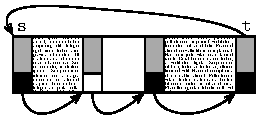
\includegraphics{arena.pdf}
\vspace{-20pt}
\caption{An arena}
\label{fig:arena}
\vspace{-15pt}
\end{wrapfigure} 

The memory manager controls the allocation and deallocation of blocks of main memory to and from client processes. The portion of memory it controls (shown in Fig.~\ref{fig:arena}) contains both free and allocated blocks. The grey cells form a cyclic chain of pointers and the white blocks in between can be allocated to clients. Since blocks are word-aligned, the least significant bit in each pointer is redundant, and is hence employed to signal the availability of the following block. In the figure, black and white squares indicate that this so-called `busy' bit is set and, respectively, unset. The module-level variables \s\ and \t\ respectively identify the first and last pointers in the arena. Because it is not followed by an allocatable block, the last pointer's busy bit is permanently set.

A client requests a block of $n$ bytes by calling $\malloc(n)$. For clarity of exposition we shall keep $n$ a multiple of the word size, \WORD. The routine traverses pointers until it finds a free block that is sufficiently large, returning the null pointer in the case of failure. It coalesces consecutive free blocks throughout the search. Should the block it finds be exactly the right size, a pointer to it is returned, and should it be too large, it is divided into two and a pointer to the first is returned. The client can later invoke $\free(x)$, $x$ being the address of the first cell in the block. Observe that \free\ is not parameterised by the length of the block, because the length was recorded when \malloc\ allocated it.


\subsection{Details of the verification}\label{sect:malloc_specifications}

\begin{figure}[t]
\[
\begin{array}{rcl}
\U[x]{y} &\EQDEF& x{<}y \land x\pto y * (x{+}1)\pto\texttt{\_} * \dots * (y{-}1)\pto\texttt{\_}  \\
\A[x]{y} &\EQDEF& x{<}y \land x\halfpto\busy{y} \\
\B[x]{y} &\EQDEF& \U[x]{y} \lor \A[x]{y} \\
\E{y}{x} &\EQDEF& x{<}y \land y\pto\busy{x} \\
\ls[x]{y} &\EQDEF& (\exists x'\ldotp \B[x]{x'} \ls{y}) \lor (x{=}y \land \emp) \\
\arena &\EQDEF& \ls[\s]{\t} * \E{\t}{\s} \\
\arena(x,n) &\EQDEF& \ls[\s]{(x{-}1)} \A{(x{+}n)} \ls{\t} * \E{\t}{\s} \\
\token(x,n) & \EQDEF& (x{-}1)\halfpto\busy{(x{+}n)} \\
\arenatoken(x,n) &\EQDEF& \boxed{\arena(x,n)} * \token(x,n)
\end{array}
\] \vspace{-10pt}
\caption{Predicates}
\label{fig:predicates}
\end{figure}

Figure~\ref{fig:predicates} defines some auxiliary predicates used in the specifications and proof. $\U[x]{y}$ describes an unallocated block between $x$ and $y$. Upon being allocated a block of size $n$ with first cell $x$, the client is also given $\token(x,n)$, which contains a half permission on the block's pointer; the manager retains the other half. We write $x\pto\busy{y}$ to mean that upon unsetting $x$'s busy bit, it would contain the address of $y$. $\E{y}{x}$ says that $y$ is the special pointer at the end of the arena that points back to $x$, the start of the arena. $\ls[x]{y}$ denotes a possibly-empty monotonically-increasing chain of pointers from $x$ to $y$ (including any unallocated blocks), the definition of which abbreviates $\B[x]{x'} * \ls[x']{y}$ to $\B[x]{x'}\ls{y}$.

\begin{figure}[tb]
\renewcommand{\arraystretch}{1.1}
\[
\begin{array}{llclcl}
\text{{\sf Coalesce}:} &\quad\qquad \U[a]{b}\U{c} & \quad \rightsquigarrow &\quad \U[a]{c} & \quad\mid &\quad \ls[\s]{a} \\
\text{{\sf AllocateEntire}:} &\quad\qquad \U[a]{b} & \quad\rightsquigarrow &\quad \A[a]{b} & \quad\mid &\quad \ls[\s]{a} \\
\text{{\sf AllocatePart}:} &\quad\qquad \U[a]{b} & \quad\rightsquigarrow &\quad \A[a]{(b{-}n)} \U{b} & \quad\mid &\quad \ls[\s]{a} \\
\text{{\sf Free}:} &\quad\qquad \A[a]{b} & \quad\rightsquigarrow & \quad \U[a]{b} & \quad\mid &\quad \ls[\s]{a} 
\end{array}
\]
\vspace{-10pt}
  \caption{Main actions}
  \label{fig:main_actions}
\vspace{-7pt}
\end{figure}

\begin{wrapfigure}{R}{35mm}
\small
\centering
\vspace{-5pt}
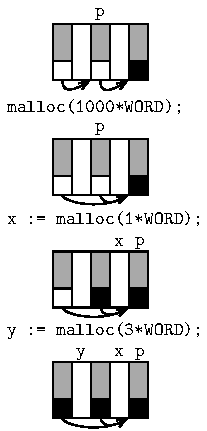
\includegraphics{bug.pdf}
\vspace{-15pt}
\caption{The bug}
\label{fig:bug}
\vspace{-40pt}
\end{wrapfigure} 
Figure~\ref{fig:main_actions} formalises the ways in which the internal heap of the module may be mutated by clients calling \malloc\ and \free. Only one routine can execute at once, so it would suffice to list a single action for each. We prefer to split them into several simple actions. The first coalesces two consecutive free blocks. The second allocates an entire block to a client, while the third allocates just the initial part. The fourth frees a block. The context $\ls[\s]{a}$ ensures that the blocks that are acted upon are really in the arena. {\sf G} is the union of all these actions.

\subsection{A (faulty) optimisation}\label{sect:mallocbug}

The following bug was discovered during the verification process.

The manager maintains a global variable {\tt p} (named {\tt allocp} in the original source code) that, after a block is allocated, is pointed to the successive block, and after a block is freed, is pointed to that block. It serves to identify a good place for the next call to \malloc\ to begin its search. The implementation does not update {\tt p} if allocation fails, however, and therein lies the bug: {\tt p} \emph{should} be updated in case the block to which it points has been coalesced with its predecessor, lest it be left pointing inside a block.

Figure~\ref{fig:bug} demonstrates how this bug could wreak havoc. Our contrived arena contains just two one-word blocks, both of which are free, and {\tt p} initially points to the second. The first \malloc\ call fails, but has the side-effect of leaving {\tt p} inside the coalesced block. We then allocate a small block at {\tt x}, before wrapping around to the start of the arena and allocating a larger block at {\tt y}, thereby reaching a situation in which the contents of the smaller block is allocated twice.

The discovery of this bug was prompted by the failure of the invariant $\ls[\s]{\p}$, which states that \p\ identifies a valid pointer in the arena. We have successfully executed our exploit to confirm that the bug is real.

\subsection{Other issues}\label{sect:malloc_otherissues}

There are several other issues involved in the implementation and verification of the memory manager, which we explain now. These issues have been sidestepped so far in order to focus on the crucial parts of the verification.
\begin{johnlist}

\johnitem{Allocation failure}
To handle the case where \malloc\ fails, its postcondition should be disjoined with the following assertion: $\floor[{\sf G}]{\,\boxed{\arena}\,} * \x{=}0$.

\johnitem{Extending the arena}
Once the search for a block has exhausted the arena, \malloc\ invokes \sbrk\ to ask the system for another block of memory. This block will be located at an address above \t\ because, in Version~7 Unix, memory allocated via \sbrk\ is never returned. The following three actions should be added to {\sf G}, to formalise these calls to \sbrk:\footnote{We are now treating module-level variables more carefully: the variable \t\ is modelled as a heap cell at address \amp\t, thus allowing  its value to be altered by these actions.} 
\[
\small
\begin{array}{@{}ll}
\text{{\sf ExtendGap}:} 
&\ \amp\t{\mapsto}t * \E{t}{\s} * \brk(b) \land b{>}t{+}1 \ \rightsquigarrow \ \amp\t{\mapsto}t' * \A[t]{b}  \U{t'} * \E{t'}{\s} * \brk(t'{+}1) \\[2pt]
\text{{\sf ExtendNoGap}:}
&\ \amp\t{\mapsto}t * \E{t}{\s} * \brk(t{+}1) \ \rightsquigarrow \ \amp\t{\mapsto}t' * \U[t]{(t{+}1)} \U{t'} * \E{t'}{\s} * \brk(t'{+}1) \\[2pt]
\text{{\sf AdvBreak}:}
&\ \brk(b) \ \rightsquigarrow \ \exists n{>}0 \ldotp \brk(b{+}n)
\end{array}
\]
The first extends the arena with a new block, leaving a gap that is filled with an unfreeable dummy block to maintain the illusion of a contiguous arena. The second is similar, but without the gap. The third action, which advances the `break value' (the cell at which the next successful call to \sbrk\ will return a block), is kept distinct to reflect that it may be performed in other situations.

\johnitem{An issue with dummy blocks}
When the arena is extended via the {\sf ExtendGap} action, the resulting gap is filled with a dummy block that is permanently allocated. In order to allocate such a block, we need to hand the caller the $\token$ predicate, yet there is no client in this situation. We thus add a $\true$ predicate to the arena, which can `soak up' these spare tokens. Considering this and the previous points, the arena (see Fig.~\ref{fig:predicates}) can be more precisely defined as follows:
\[
\arena \EQDEF \exists s,t,b \ldotp \true * \amp\s{\mapsto}s * \amp\t{\mapsto}t *\ls[s]{t} * \E{t}{s} * \brk(b) \land t<b
\]
\end{johnlist}

\section{Related Work}

Explicit stabilisation arose out of `mid stability' \cite[\S 4.1]{viktor_thesis}, a variation of RG reasoning that places stability checks not on the pre and postconditions of basic commands, but at the points of sequential and parallel composition instead. This more strategic placement eliminates redundant checks, and also allows libraries comprising just one basic command to be verified without considering stability. Our parametric proof system (Fig.~\ref{fig:paraspec_rules}) extends this to \emph{all} library functions (and encodes mid stability soundly and completely).

RG-style reasoning has been used before to verify concurrent library code (e.g.~\cite{calvin}). The specifications of that approach involve a particular rely, whereas our parametric specifications do not require a particular rely to be instantiated.

RG has also furnished proofs of sequential modules before (e.g.~\cite{gretayorsh}), but we believe ours to be the first that hides the module's internal interference. The {\sc InfoHiding} rule that enables this feat is related to the hypothetical frame rule \cite{sepinfhiding}: the latter rule hides the module's \emph{state} from the client, while ours hides the module's \emph{interference}. Perhaps the hypothetical frame rule could be used to remove the $\boxed{\arena}$ predicate from the verification given in Fig.~\ref{fig:malloc_client}, thus revealing to the client neither the module's state nor its internal interference.

SAGL \cite{sagl}, like RGSep, is a descendant of RG and separation logic, to which explicit stabilisation could also be applied. Local Rely-Guarantee (LRG) \cite{lrg} is a third descendant that addresses an inherent flaw in the modularity of its siblings: that the shared heap must be globally known. It defines a $*$ operator over interference, which allows the shared heap to be split into portions that are shared between just a few threads. The application of explicit stabilisation to LRG could simplify the verification of clients that invoke multiple modules, for our approach currently handles only one.

Explicit stabilisation can be seen as a bridge between theory and implementation: tools, such as SmallfootRG \cite{smallfootrg}, that automate RG-style reasoning may defer stability checks rather than perform them at the point of rule application, and explicit stabilisation can help to formalise this `lazy' approach. We have not considered the implementation of stabilisation; this issue is explored in \cite{automaticstability}.

\section{Conclusion}
We have proposed explicit stabilisation as a new way to deal with stability in RG reasoning. The central idea is to record information about an assertion's stability into its syntactic form. The main benefits are in modular reasoning:
\begin{johnlist}
\johnitem{Library code can be verified independently of clients} In Sect.~\ref{sect:modularity_solution}, we showed how an approach based upon explicit stabilisation enables RG reasoning to verify concurrent library code. Essentially, the stabilisation in the library's specification is evaluated so lazily that it actually becomes an obligation of the client.
\johnitem{Client code can be verified independently of a sequential module} We showed in Sect.~\ref{sect:rgsep} how the application of explicit stabilisation to RGSep gives rise to an {\sc InfoHiding} rule that allows a sequential module to hide its internal interference from its clients. Such information hiding is crucial for modular reasoning, because it allows the specification of a client to be reused, even despite changes to the specification of this internal interference. Section~\ref{sect:malloc} demonstrated this reasoning by verifying a memory manager.
\end{johnlist}
It would be interesting to investigate whether these two forms of modularity can be combined; that is, can we verify both a library and its clients, modularly, at the same time? It looks feasible. The specification for the library in Sect.~\ref{sect:modularity_solution} used explicit stabilisation with an arbitrary rely $R$, which became specific for each client in turn. Meanwhile, the specifications for the memory manager in Sect.~\ref{sect:malloc} used explicit stabilisation with the specific $G$ of the module, which was then generalised to an arbitrary $G$ for the clients, so as to provide information hiding. Perhaps a combination of these approaches would parameterise on both the rely and the guarantee? 

We also plan to apply explicit stabilisation to more advanced logics based on RG, such as LRG, Deny-Guarantee \cite{dg}, and the logic of Gotsman et al.\ for proving liveness \cite{alexey}. The notions of stability in such logics are becoming ever more demanding, so it is increasingly important to have a solid basis upon which to reason about stability. We believe explicit stabilisation provides such a basis.

\subsection*{Acknowledgements}
The idea of parameterising RG specifications on the `current rely' is due to Hongseok Yang. Richard Bornat introduced us to the malloc example. We also thank Joey Coleman, Xinyu Feng, Erica Fulbrook, Cliff Jones, Alexander Malkis, Tom Ridge and Viktor Vafeiadis for feedback and helpful discussions. This work was supported by EPSRC grant F019394/1. Parkinson is supported by a Royal Academy of Engineering/EPSRC fellowship.

\bibliographystyle{abbrv}
\bibliography{expstab} 

\appendix

\section{Source code of Unix V7 memory manager}\label{sect:mallocsource}

Abridged and corrected. Retrieved from the Unix Heritage Society.\footnote{\url{http://minnie.tuhs.org/UnixTree/V7/usr/src/libc/gen/malloc.c.html}}

\lstset{
  language=C,
  columns=fixed,
  fontadjust=true,
  mathescape=true,
  basewidth=0.47em,
  basicstyle=\ttfamily\fontsize{8pt}{9pt}\selectfont,
  showstringspaces=false
} 
\begin{multicols}{2}
\begin{lstlisting}
#define WORD sizeof(st)
#define BLOCK 1024
#define testbusy(p) ((int)(p)&1)
#define setbusy(p) (st *)((int)(p)|1)
#define clearbusy(p) (st *)((int)(p)&~1)
struct store { struct store *ptr; };
typedef struct store st;
static st s[2]; /*initial arena*/
// static struct store *allocp; (bug removed)
static st *t;   /*arena top*/
char* sbrk();
char* malloc(unsigned nbytes) {
  register st *p, *q;
  register nw;  static temp;
  // omitted: initialisation code
  nw = (nbytes+WORD+WORD-1)/WORD;
  for(p=s; ; ) {
    for(temp=0; ; ) {
      if(!testbusy(p->ptr)) {
        while(!testbusy((q=p->ptr)->ptr)) 
          p->ptr = q->ptr;
        if(q>=p+nw && p+nw>=p) goto found;
      }
      q = p; p = clearbusy(p->ptr);
\end{lstlisting}
\begin{lstlisting}
      if(p>q) ;
      else if(q!=t || p!=s) return 0;
      else if(++temp>1) break;
    }
    temp = ((nw+BLOCK/WORD) 
              /(BLOCK/WORD))*(BLOCK/WORD);
    q = (st *)sbrk(0);
    if(q+temp < q) return 0;
    q = (st *)sbrk(temp*WORD);
    if((int)q == -1) return 0;
    t->ptr = q;
    if(q!=t+1) t->ptr = setbusy(t->ptr);
    t = q->ptr = q+temp-1;
    t->ptr = setbusy(s);
  }
found:
  if(q>p+nw) ((st *)(p+nw))->ptr = p->ptr;
  p->ptr = setbusy(p+nw);
  return((char *)(p+1));
}
free(register char *ap) {
  register st *p = ((st *)ap)-1;
  p->ptr = clearbusy(p->ptr);
}
\end{lstlisting}
\end{multicols}


\end{document}